51. \begin{figure}[ht!]
\center{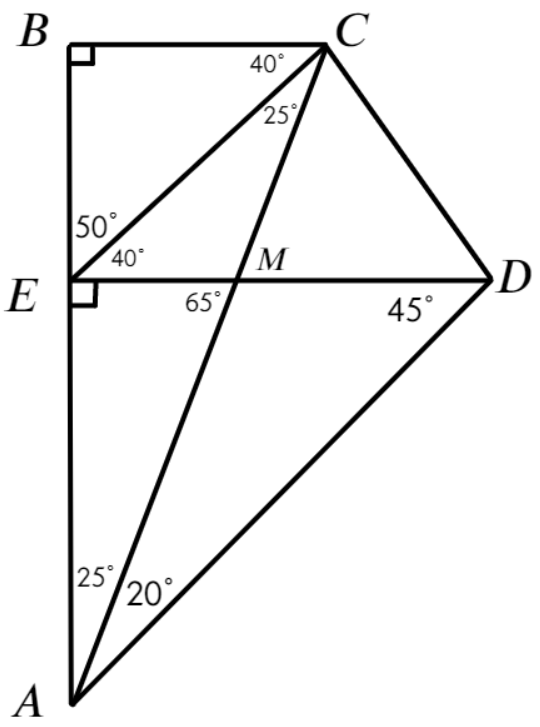
\includegraphics[scale=0.35]{g51.png}}
\end{figure}\\
Посчитаем углы на картинке: $\angle BEC=90^\circ-40^\circ=50^\circ,\ \angle CEM=90^\circ-50^\circ=40^\circ,\ \angle EAD=90^\circ-45^\circ=45^\circ,\ \angle EAC=90^\circ-65^\circ=25^\circ,\ \angle ECM=180^\circ-90^\circ-40^\circ-25^\circ=25^\circ.$ Таким образом по паре равных углов имеют треугольники $CEA$ и $EAD,$ а значит они равнобедренные и $CE=AE,\ AE=ED,$ поэтому и $CE=ED.$ Тогда треугольник $CED$ является равнобедренным, как и треугольник $CEA,$ ч.т.д.\\
